\chapter{Introduction}

Many of us are familiar with the image of the periodic table of the elements (Figure \ref{fig:periodictable}) - it is a list of the fundamental substance which constitutes the matter around us. It is differing combinations of these elements which form everything from the water and DNA in our body to the composition of stars in the far galaxy. A handful of these elements have been known since antiquity and led to ew elements began to be discovered and scientists were in hopes of somehow classifying these into a common framework.  

\begin{figure}[hb!]
\centering
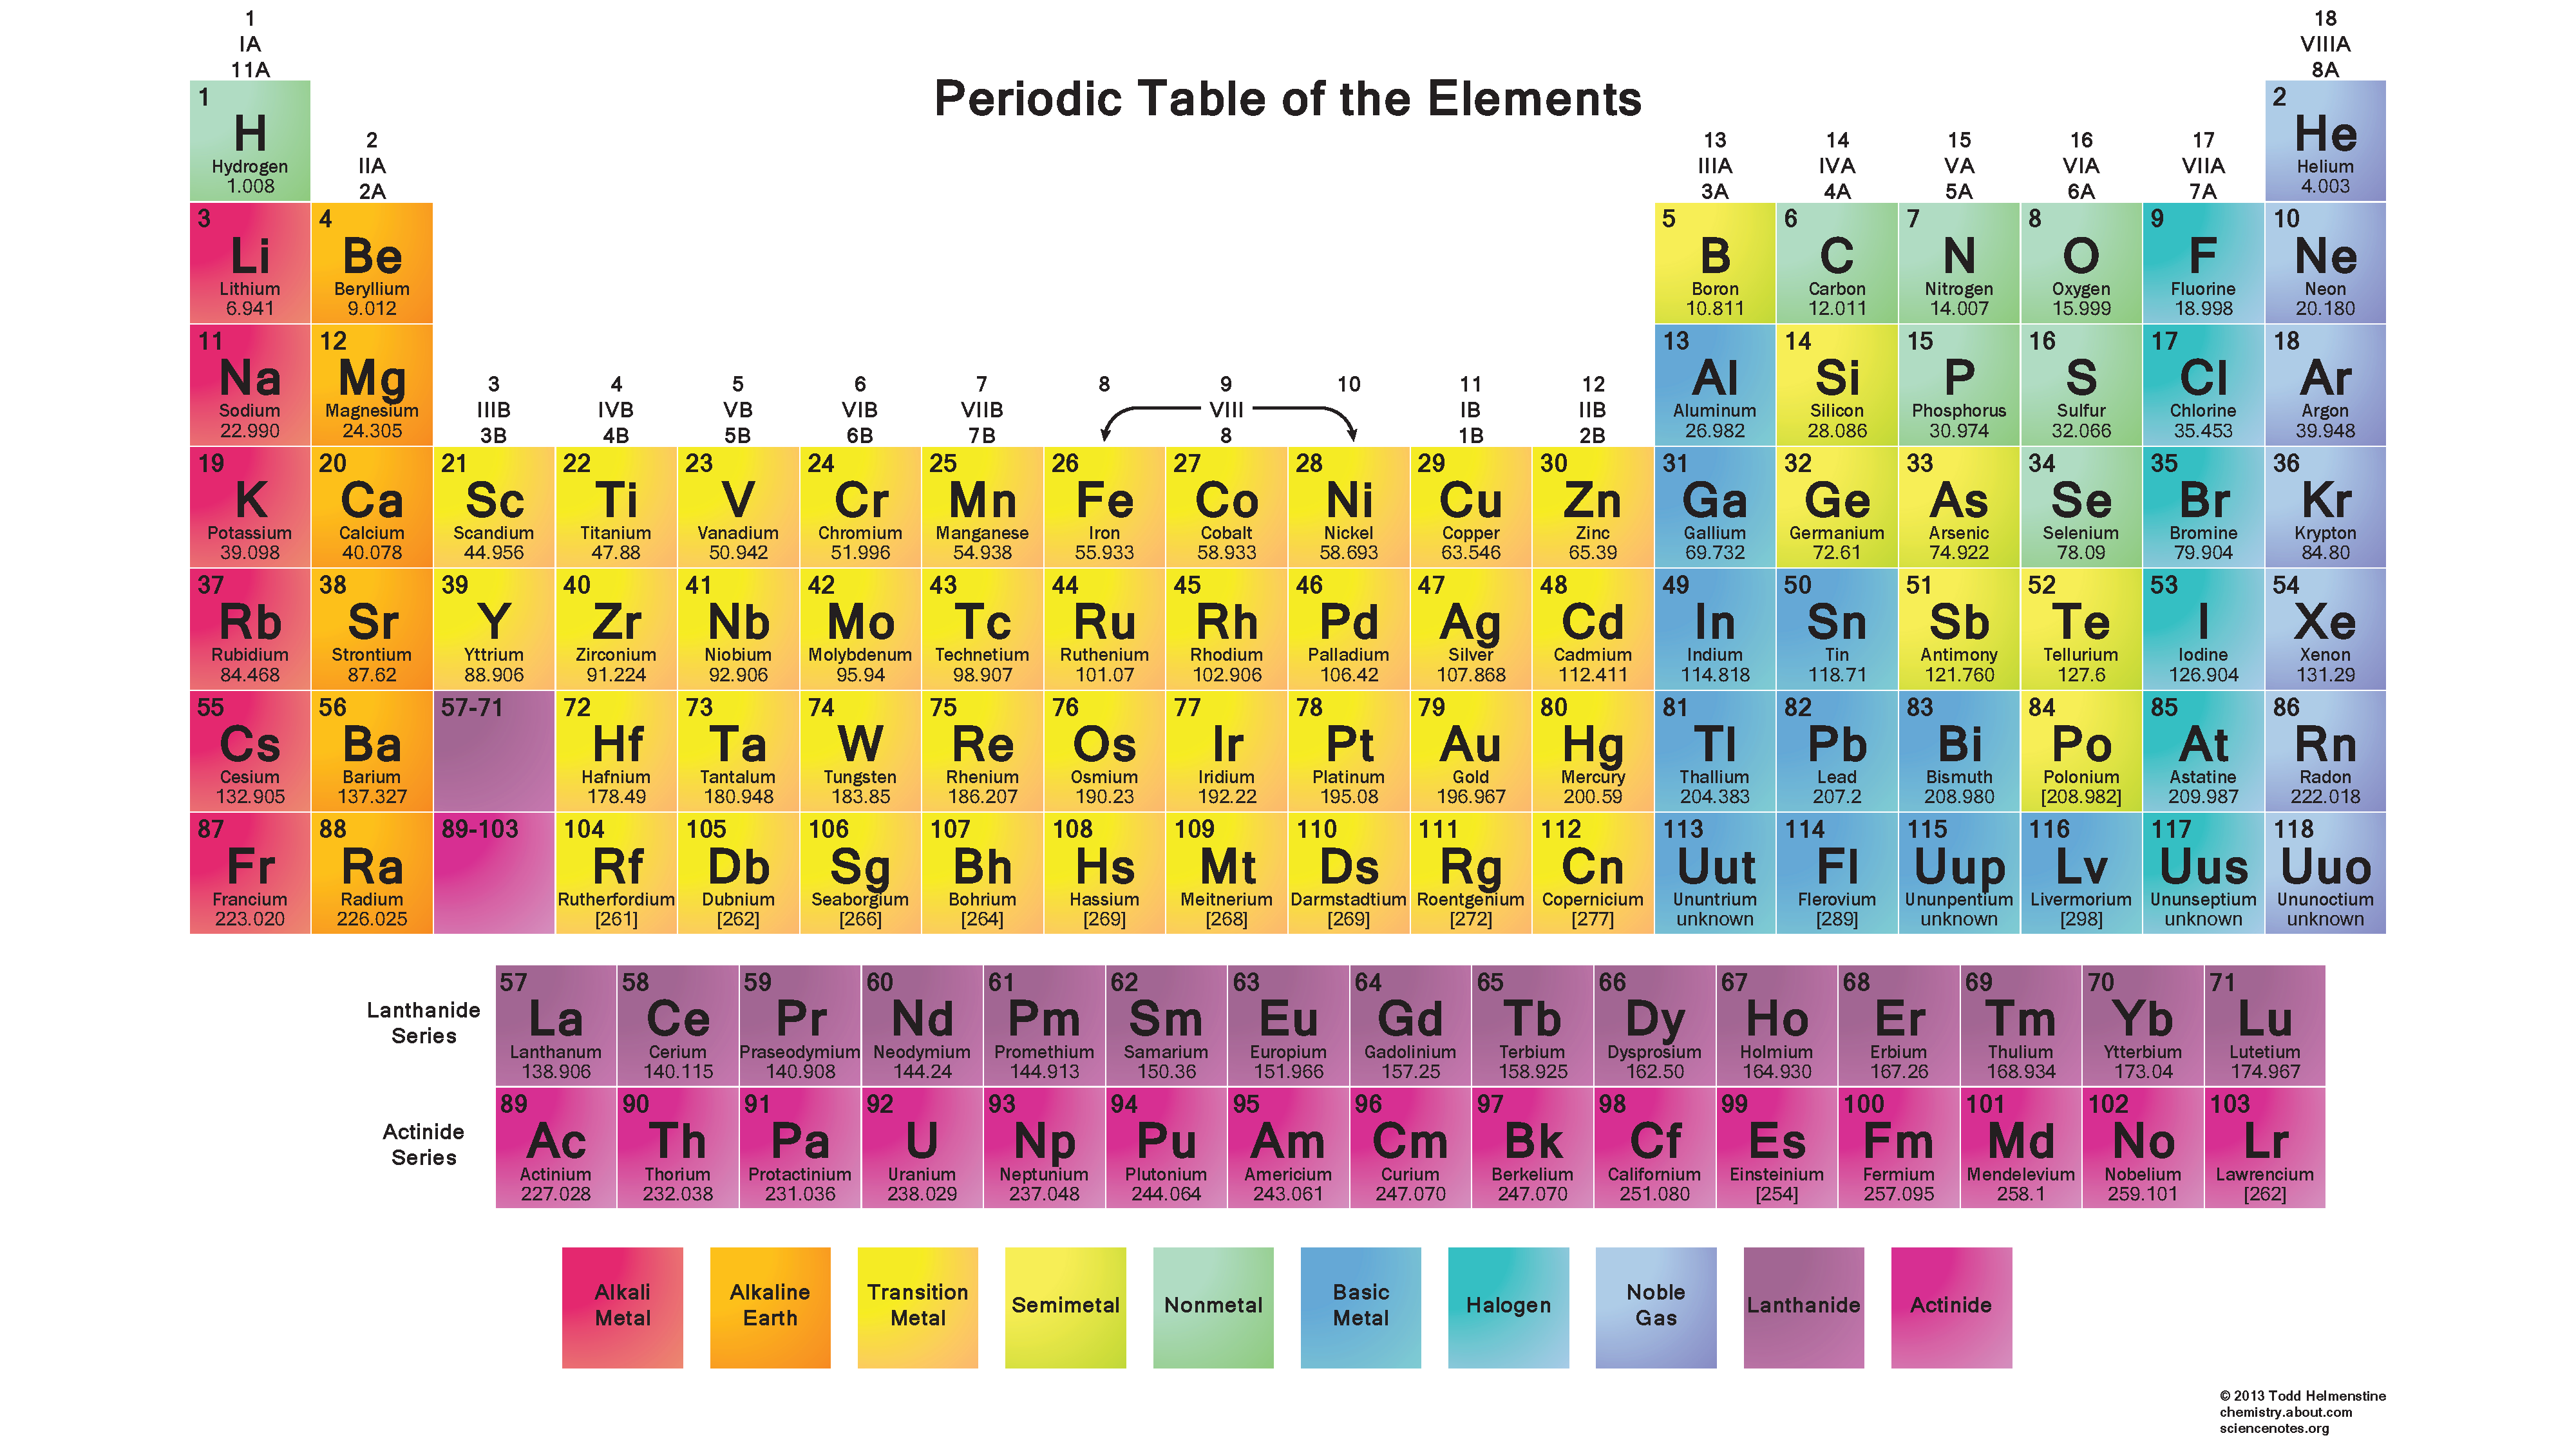
\includegraphics[width=0.8\textwidth]{figs/PeriodicTable.pdf}
\caption{The periodic table of elements.}
\label{fig:periodictable}
\end{figure}

\begin{figure}[htbp]
\centering
\includegraphics[width=0.6\textwidth]{figs/StandardModelofElementaryParticles.pdf}
\caption{The particles of the Standard Model.}
\label{fig:sm}
\end{figure}

But there is no reason to expect that the atoms of the Periodic Table th

But the elements themselves are made of more fundamental ``atoms'' described by the Standard Model of particle physics, the current knowledge is summarized in another table, seen in Figure \ref{fig:sm}.


The 'completion' or 'success' of the periodic table begs the question of whether the atoms which constitute the elements are themselves composite of smaller or more fundamental objects.


A description of the Standard Model is presented in Chapter \ref{chap:sm}. A description of Supersymmetry is presented in Chapter \ref{chap:mssm}. A description of the Large Hadron Collider (LHC) is presented in Chapter \ref{chap:lhc}. A description of the CMS detector is presented in Chapter \ref{chap:detector}. A description of the physics event reconstruction is presented in Chapter \ref{chap:eventreco}. A description of the physics analysis is presented in Chapter \ref{chap:analysis}. The conclusions are discussed in Chapter \ref{chap:conclusions}.
